A common approach for MIL is to use some form of dissimilarity measure in the classification of new bags. 
For instance-level information, the dissimilarity is measured between the instances in a bag and instances in labelled bags or prototypes. 
An example is the Harrington distance, and its variants. 
For bag-level information, the dissimilarity is measured between the bag as a whole and labelled bags or prototypes. 
{\color{red} In the bag space, the dissimilarity is calculated based on the instance values.}
In the embedded space, the instance values are transformed to a single vector (e.g. population mean and variance), and a single-instance dissimilarity measure can be used. 
Hybrid versions also exist, see e.g. {\color{green} Chepuliga (2016)}. 

We here introduce two new approaches that has not been studied in the MIL context: 
(1) Divergence-based dissimilarity measures. 
(2) Bag-to-class dissimilarities. 

A divergence function (or simply divergence) is a measure of dissimilarity between two probability distributions.
Divergences are not distance functions in the mathematical definition, as they don't necessarily fulfil the symmetry or the triangle inequality properties. 
Common divergences are the Kullback-Leibler information, the Bhattacharrya distance, etc. 
There are no common properties that a function has to fulfil to be called a divergence, but many divergences have known properties, and are categorised accordingly. 
Because dissimilarity between probability distributions is not uniquely defined, but very much depends on the problem at hand, there is a huge range of divergences. 
In that aspects, divergences are suited to solve MI problems if the proper divergence can be matched. 
% In the MIL context, the instances of a bag form the basis of a probability distribution estimate, and then a divergence can be applied. 
Let 
\begin{align}
  D(P_{bag}, P_{ref})\, ,
\end{align}
where $P_{bag}$ is the probability distribution of the bag that we want to classify, and $P_{ref}$ is the reference distribution, be a divergence. 
$P_{ref}$ can be any distribution, but would typically be that of labelled bags, classes, or prototypes. 

The bag-to-class dissimilarity has not been used in MIL, although there are obvious advantages:
For one, the computation time decreases when the dissimilarity is calculated only between a bag and the classes, compared to pairwise dissimilarities between a bag and all labelled bags. %  or prototypes. 
Generally, we do not assume that bags in a class are equal, and therefore, after calculating the dissimilarities between the new bag and the labelled bags, a second step must be decided upon: how many bags will influence the classification, and how are they weighted.

A bag-to-class approach can also be used without a divergence, but we will proceed with the divergence approach. 

For a new bag, we want to measure $D(P_{bag},P_{\cpos})$ and/or $D(P_{bag},P_{\cneg})$.
$P_{\cpos}$ is not equal to any $P_{bag}$ of the positive class, but rather all possible bag distributions of the positive class with their probability of occurrence taken in mind. 
A bag's distribution is then one of the possible distributions of that class. 
Therefore, symmetry of the divergence is not a requirement.

Back to the example of tissue images, we can illustrate it as follows. 
\begin{figure}[!h]
  \centering
    \includegraphics[height = 0.3\textheight]{/Volumes/kam025/Documents/Figures/Divergence_Manuscript/tumourVSnormal.pdf}
\end{figure}
The class of tumour images and the class of normal images overlap, but there is a larger difference between the two classes for pixels values in the tumour range than in the normal range. 
The pdf of a bag will not resemble the pdf of either classes of images. 
\begin{figure}[!h]
  \centering
    \includegraphics[height = 0.3\textheight]{/Volumes/kam025/Documents/Figures/Divergence_Manuscript/tumVSnorm.pdf}
\end{figure}

If we could accurately estimate $f^+(x)$, the distribution of the tumour pixels, and $\pi_{bag}^+$, the proportion of tumour pixels in an unlabelled image, we could treat this as a count-based assumption and classify accordingly. 
However, by using the pdfs directly, without explicitly estimating the parameters in the different levels of the Bayes' hierarchy, we can possibly make more accurate estimates. 
In this example, we see that the overlapping area between bag and class is fairly similar for both classes in the normal pixel range. 
But for the tumour pixel range, the difference is larger. 
However, since the proportion of normal pixels is larger than that of tumour pixels, there is a risk of ignoring this if we measure dissimilarity by overlapping areas, as e.g. the Bhattacharyya distance does.
A different way of measuring dissimilarity is by distribution ratio $f_{bag}(x) /f_\cpos(x)$ and $f_{bag}(x) /f_\cneg(x)$.
Let $D(f_{bag}(x), f_\cpos(x)$) denote the dissimilarity measured from $f_{bag}(x)$ to $f_\cpos(x)$.

The Kullback-Leibler information from $f_{bag}(x)$ to $f_\cpos(x)$ is defined as
\begin{align}
  D_{KL}(f_{bag},f_\cpos) = \int f_{bag}(x) \log \frac{f_{bag}(x)}{f_\cpos (x)} dx.
\end{align}
It is non-symmetric, and it is an $f$-divergence. 

The Kullback-Leibler information is suited for the tissue image example, where the discriminative power lies with the tumour pixels, since the ratio of positive bag to negative class is large for tumour pixels. 

If the proportion of tumour pixels in the normal image class is zero (standard MI assumption), the Kullback-Leibler information attains its maximum value (infinity) between a tumour image and the normal image class. 


% A class can be seen as a prototype, and in that case, bag-to-class will be the minimum number of prototypes. 
% We propose a dissimilarity measure for bag-to-class comparison, based on the divergence between two probability distributions. 
 % We will also shortly discuss divergence for bag-to-bag comparison. 

See e.g. {\color{green} Mollersen et al} for properties of some common divergences. 

%Let $\mathcal{X}_{pos>{bag,pos}}$ be the region where $p_{pos}(x)>p_{bag,pos}(x)$. 
%Then $\mathcal{X}_{pos>{bag,pos}} \geq \mathcal{X}_{pos \leq {bag,pos}}$, 
%meaning that the region where $p_{pos}$ is greater than $p_{p\_ bag}$ is bigger than the opposite. 
%This comes from the hierarchical nature of $P_{pos}$, where $\theta_{pos} = [\pi_{pos} \,\,\,\theta_+ \,\,\,\theta_-]$ has a distribution, and $p_{p\_ bag}$ is uniquely defined by the $\theta_{pos}$ sample. 
An illustration
\begin{figure}[!h]
  \centering
  \begin{subfigure}{}
    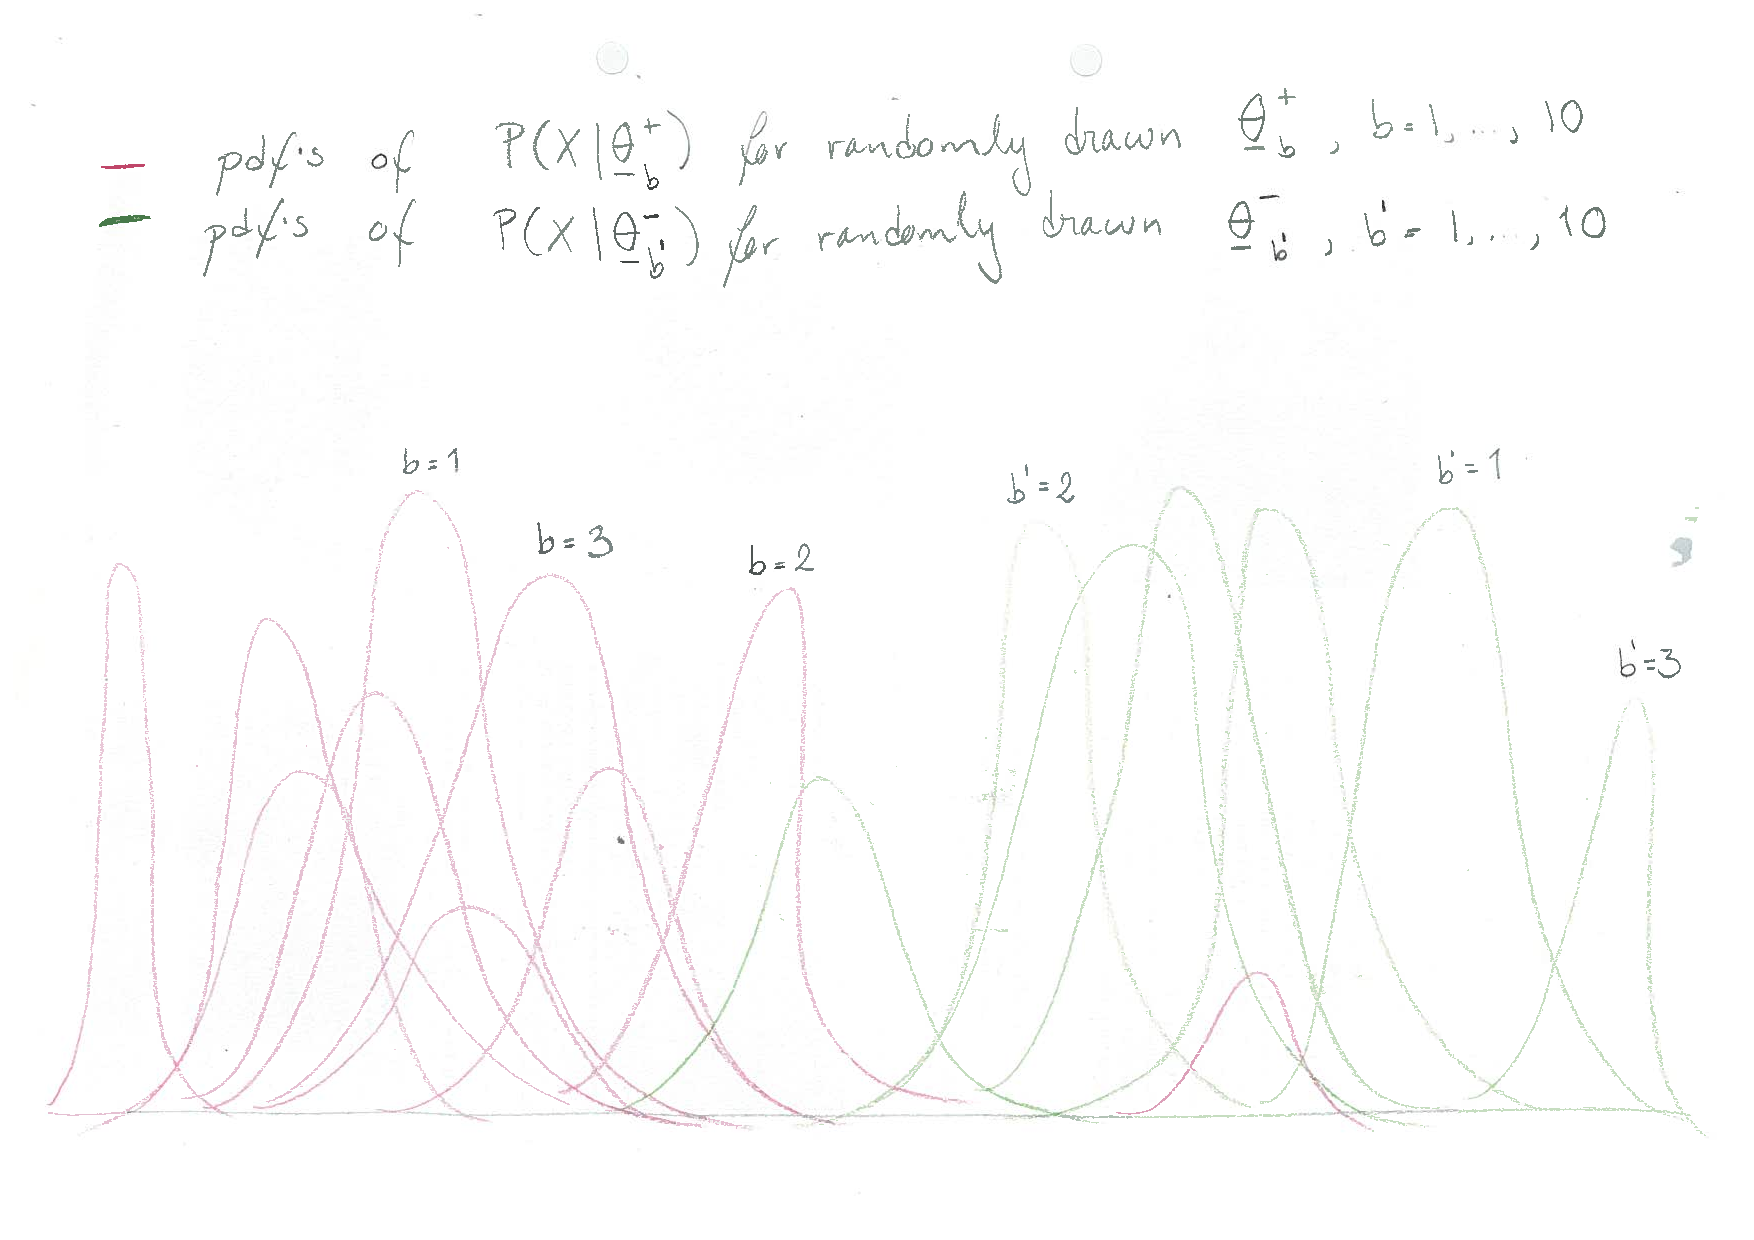
\includegraphics[height = 0.3\textheight]{/Volumes/kam025/Documents/Figures/Divergence_Manuscript/distrs.pdf}
  \end{subfigure}    
  \begin{subfigure}{}
    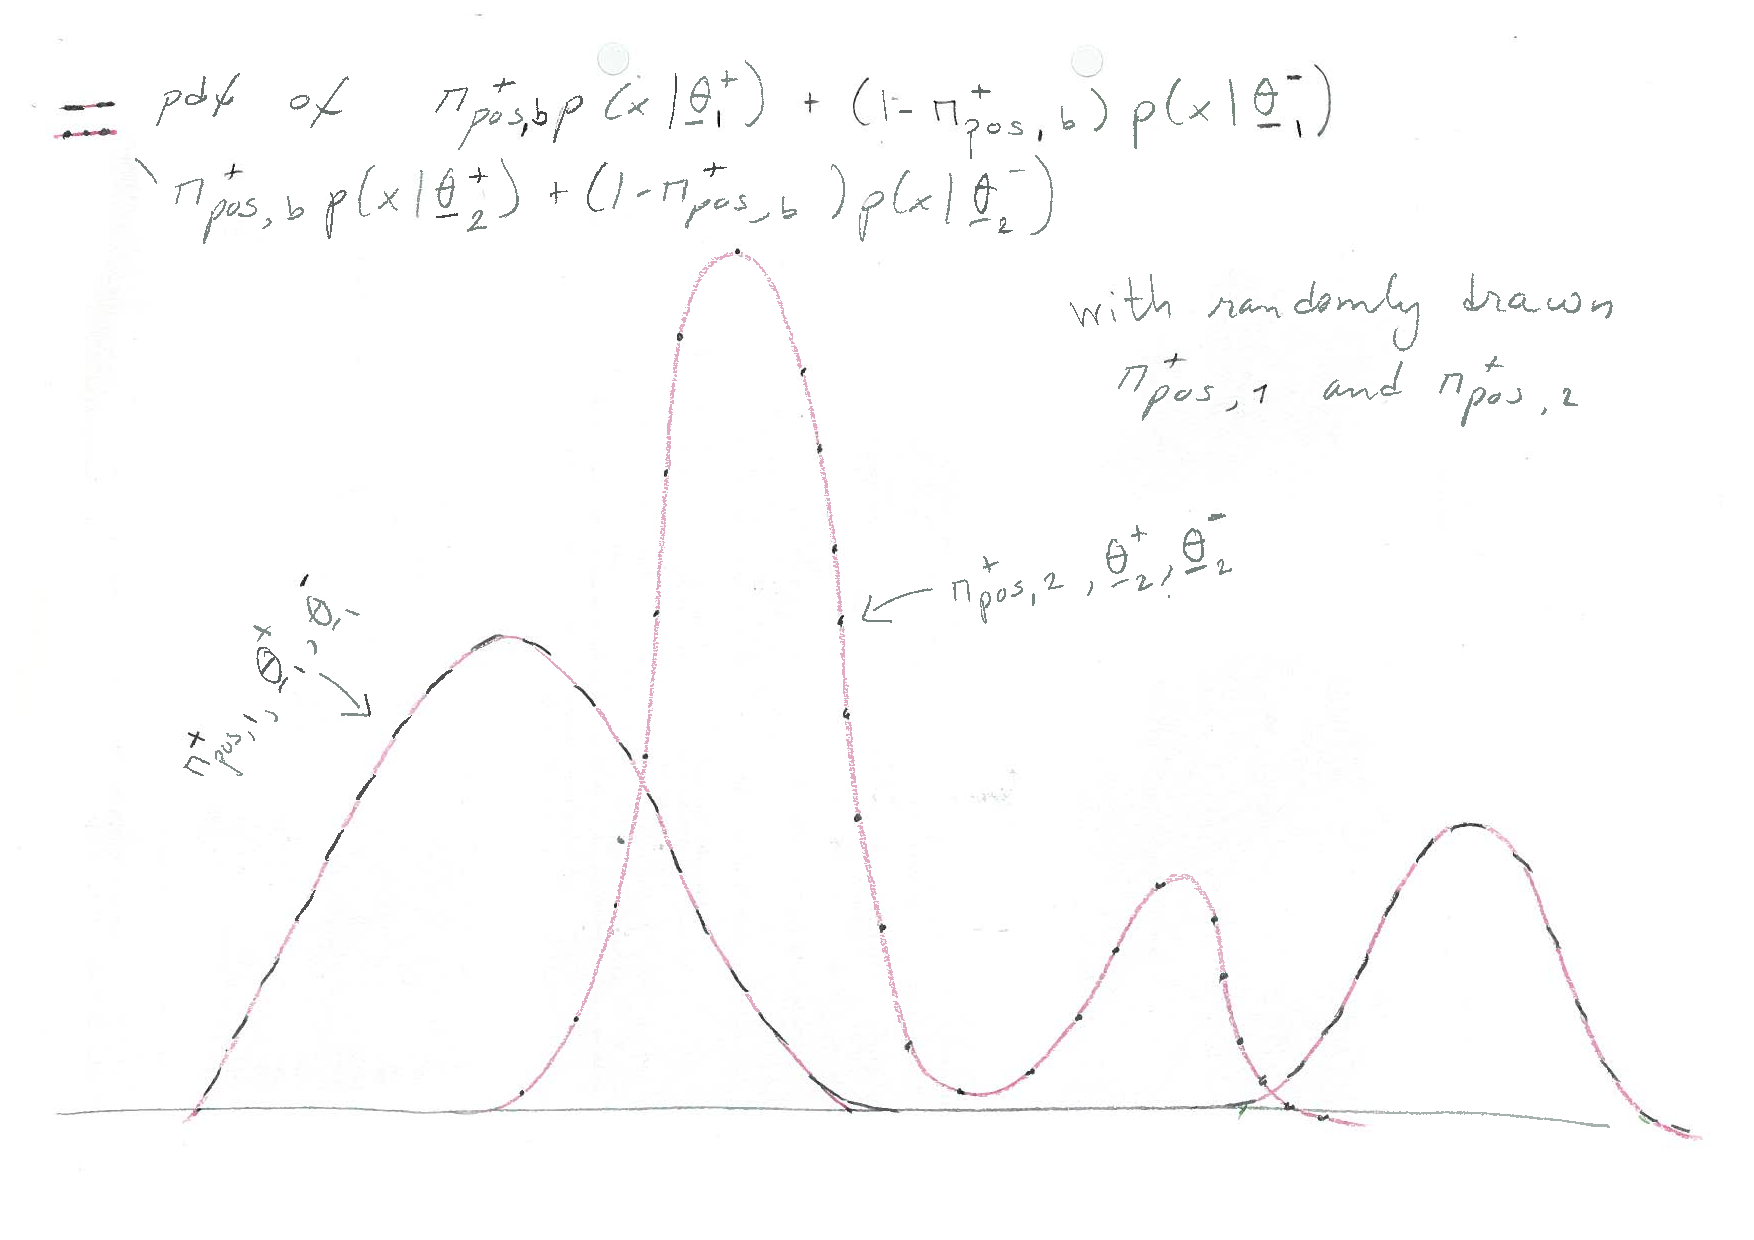
\includegraphics[height = 0.3\textheight]{/Volumes/kam025/Documents/Figures/Divergence_Manuscript/pos.pdf}
  \end{subfigure}
  \begin{subfigure}{}
    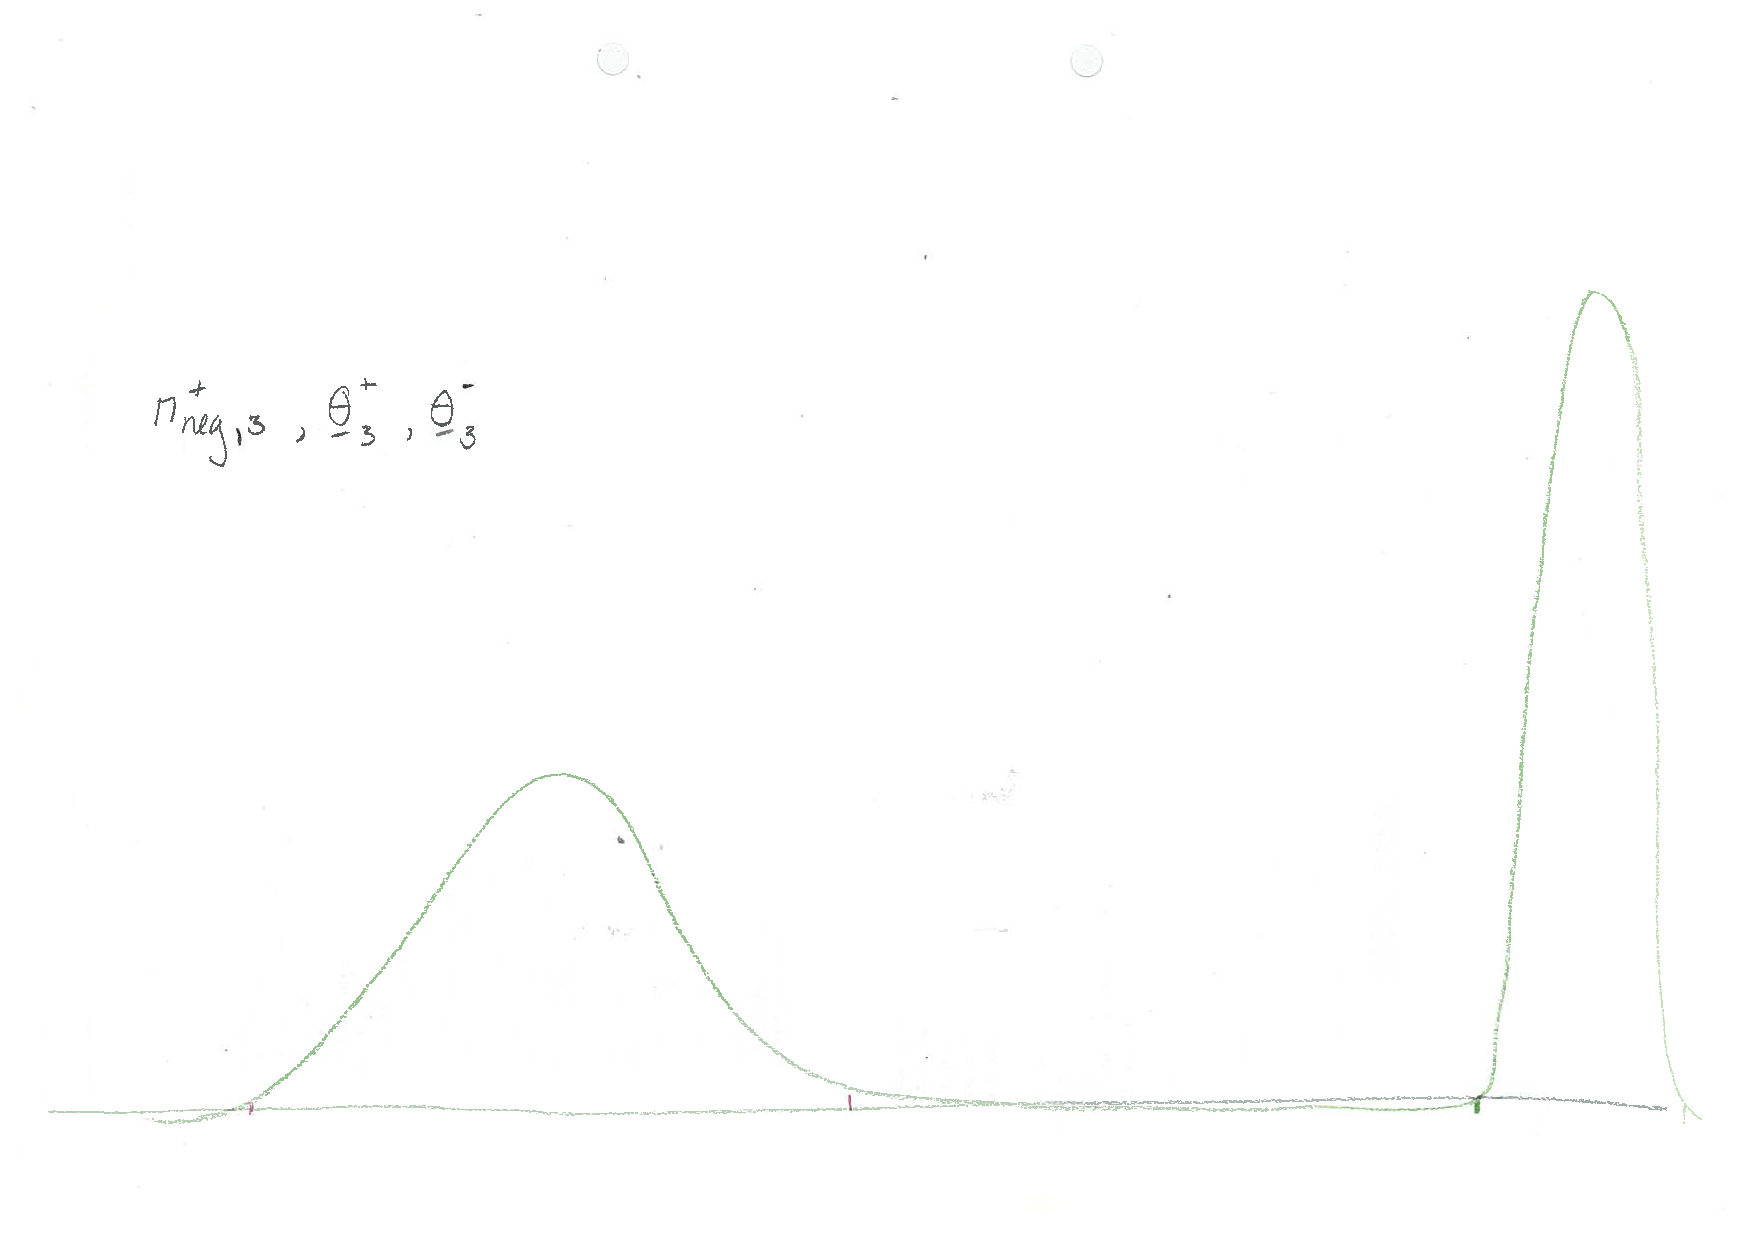
\includegraphics[height = 0.3\textheight]{/Volumes/kam025/Documents/Figures/Divergence_Manuscript/neg.pdf}
  \end{subfigure}
\end{figure}

The goal is to pick a divergence that is able to discriminate between a positive and a negative bag by measuring the dissimilarity to $P_{pos}$ and/or $P_{neg}$.
%Let $\mathcal{X}_{pos > neg}$ be the region where $p_{pos}(x) > p_{neg}(x)$. 
%Unless $p_{pos} = p_{neg}$ we have $\mathcal{X}_{pos > neg}$ nonempty, which gives $\mathcal{X}_{pos < neg}$ nonempty, whereas $\mathcal{X}_{pos = neg}$ might be empty or not. 

%The Kullback-Leibler information (KL inf),
%\begin{align}
%  d_{KL}(p_{bag},p_{neg}) = \int_\mathcal{X} p_{bag}(x) \log \frac{p_{bag}(x)}{p_{neg}(x)} dx,
%\end{align}
%is a non-symmetric $f$-divergence.
%The log ratio function gives a positive contribution whenever $p_{bag}>p_{neg}$, and a negative contribution for $p_{bag}<p_{neg}$, and zero contribution for $p_{bag} = p_{neg}$.
%A large positive contribution for $p_{bag} >> p_{neg}$ and $p_{bag} >> 0$, which means that if $p_{bag}$ is outside the range of $p_{neg}$, the dissimilarity approaches infinity. 
%This is a suitable property, because if $p_{bag}/p_{neg} \rightarrow \infty$, the probability the parameters of $p_{bag}$ are not sampled from the negative class. 
A simple straightforward classification is then
\begin{align}
  \frac{D_{KL} (f_{bag},f_{\cpos})}{D_{KL} (f_{bag},f_{\cneg})}.
\end{align}

%Because we also assume that $\pi_{pos} > \pi_{neg}$ it follows that $p_{p \_ bag} < p_{n \_ bag}, X \in \mathcal{X}_{neg}$ and therefore 
%\begin{align}
%  \int_{\mathcal{X}_{neg}} \frac{p_{pos}(x)}{p_{neg}(x)} p_{p\_bag}(x) \log \frac{p_{p\_bag}(x)}{p_{neg}(x)} dx < \int_{\mathcal{X}_{neg}} \frac{p_{pos}(x)}{p_{neg}(x)} p_{n \_ bag}(x) \log \frac{p_{n \_bag}(x)}{p_{neg}(x)} dx
%\end{align}
%which is an unwanted property, and therefore we use only $\mathcal{X}_{pos}$.

%Like with KL inf, the log ratio function ensures large positive contributions for $p_{bag} >> p_{neg}$ when also $p_{bag} >> 0$. 
%In addition, we require that $p_{pos} > p_{neg}$ for this contribution to be large. 
%This is because if $p_{bag} >> p_{neg}$ but $p_{pos} < p_{neg}$ we have a bag whose pdf cannot be explained by the negative class, but neither by the positive class, and therefore is uninformative for classification. 
%If $p_{pos} > p_{neg}$, or even $p_{pos} >> p_{neg}$, then $D \rightarrow \infty$.
%How is this different from $d_{KL}(p_{bag},p_{pos})/d_{KL}(p_{bag},p_{neg})$?
%If $p_{bag}/p_{pos} \rightarrow \infty$ and $p_{bag}/p_{neg} \rightarrow \infty$, then the ratio will be one. 

Why not use bag-to-bag?

\begin{align}
  \frac{p_{bag,b}}{p_{bag,b'}} \rightarrow \infty
\end{align}


In practice, the distributions must be estimated from the instances of the bag, using the assumption that they are independent observations from a common underlying distribution. 
Commonly used is the EM-algorithm.
Which method to apply for distribution estimation depends on the data, especially the sparsity, previous knowledge, and requirements regarding time consumption. 
We will not go into the details, but simply use the EM-algorithm.
Assuming that the instances are observations from an underlying distribution. 


